\documentclass{../../slides-style}

\slidetitle{Развёртывание, Docker}{12.12.2024}

\begin{document}

    \begin{frame}[plain]
        \titlepage
    \end{frame}

    \section{Введение}

    \begin{frame}
        \frametitle{Docker}
        \begin{itemize}
            \item Средство для \enquote{упаковки} приложений в изолированные контейнеры
            \item Что-то вроде легковесной виртуальной машины
            \item DSL для описания образов 
            \item Публичный репозиторий
            \item Стандарт де-факто для деплоя веб-приложений
        \end{itemize}
        \begin{center}
            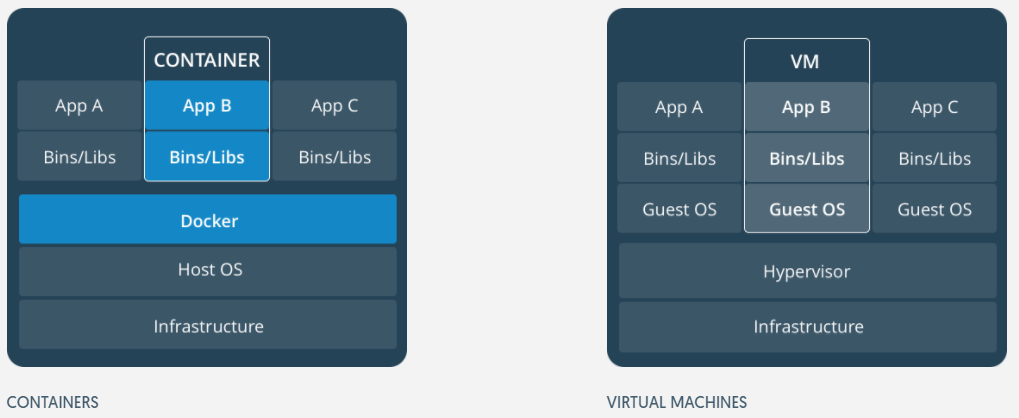
\includegraphics[width=0.7\textwidth]{docker.png}
            \attribution{\url{https://www.docker.com}}
        \end{center}
    \end{frame}

    \begin{frame}
        \frametitle{Docker Image}
        \begin{columns}
            \begin{column}{0.6\textwidth}
                \begin{itemize}
                    \item Окружение и приложение
                    \item Состоит из слоёв
                    \begin{itemize}
                        \item Все слои read-only
                        \item Образы делят слои между собой как процессы делят динамические библиотеки
                    \end{itemize}
                    \item На основе одного образа можно создать другой
                \end{itemize}
            \end{column}
            \begin{column}{0.4\textwidth}
                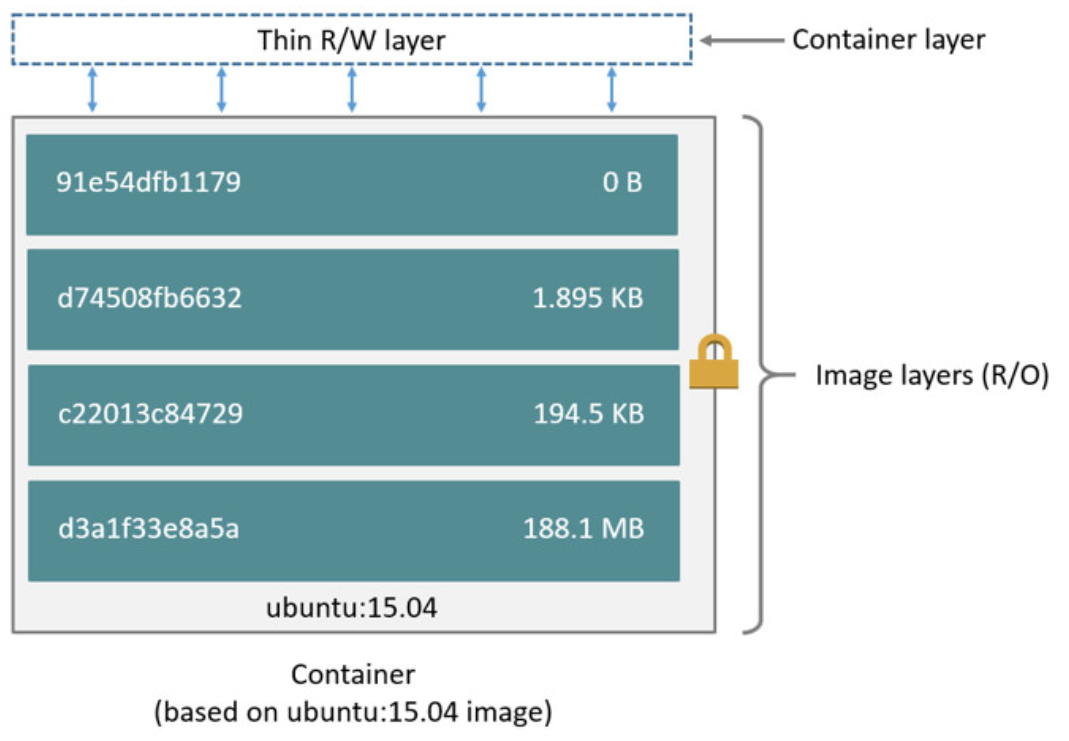
\includegraphics[width=0.9\textwidth]{dockerLayers.png}
            \end{column}
        \end{columns}
    \end{frame}

    \begin{frame}
        \frametitle{Docker Container}
        \begin{columns}
            \begin{column}{0.5\textwidth}
                \begin{itemize}
                    \item Образ с дополнительным write слоем
                    \item Содержит один запущенный процесс
                    \item Может быть сохранен как новый образ
                \end{itemize}
            \end{column}
            \begin{column}{0.5\textwidth}
                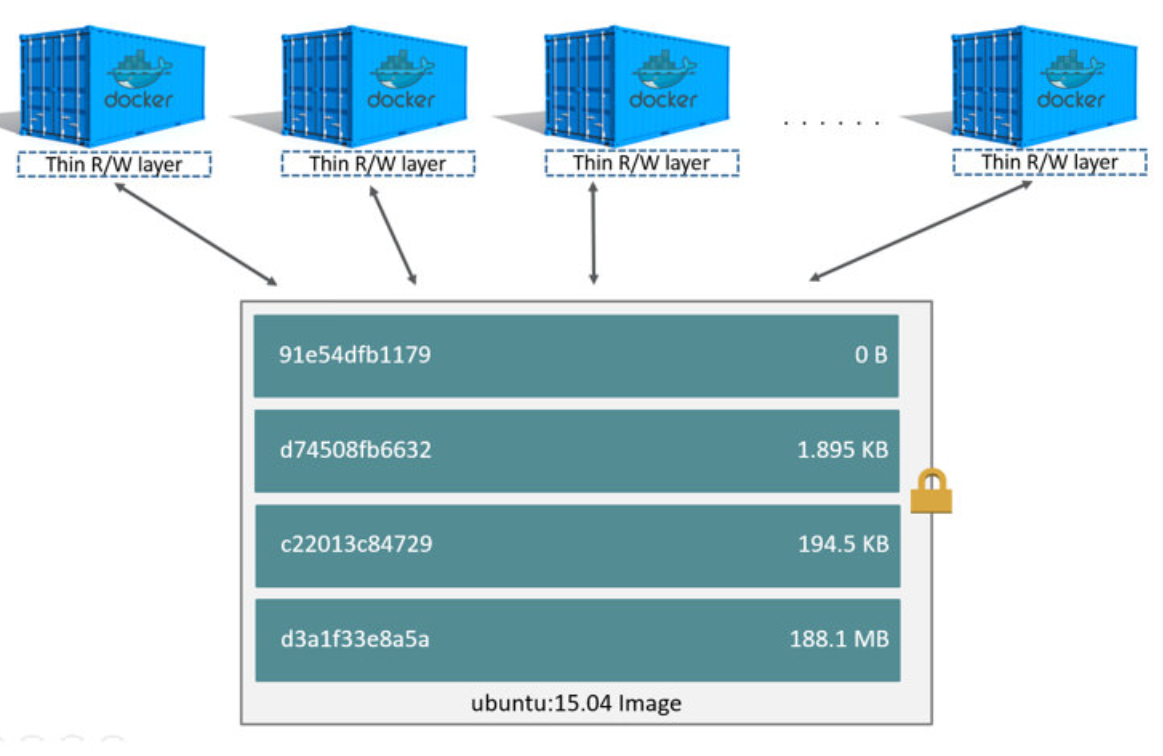
\includegraphics[width=0.9\textwidth]{dockerContainer.png}
            \end{column}
        \end{columns}
    \end{frame}

    \begin{frame}
        \frametitle{Хранение данных}
        \begin{columns}
            \begin{column}{0.5\textwidth}
                \begin{itemize}
                    \item По умолчанию все данные хранятся только в памяти
                    \item Для БД и т.п. --- volumes и bind mounts
                \end{itemize}
            \end{column}
            \begin{column}{0.5\textwidth}
                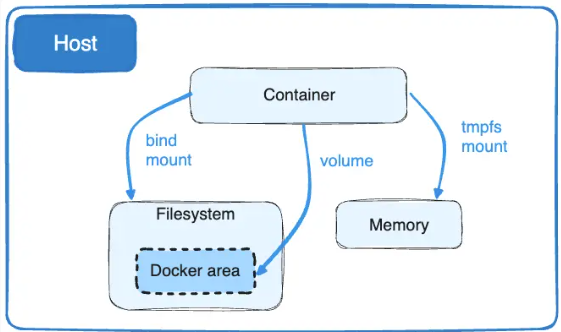
\includegraphics[width=0.9\textwidth]{persistence.png}
            \end{column}
        \end{columns}
        \begin{itemize}
            \item \mintinline{text}|docker run -d --mount source=myvol,target=/app nginx:latest|
        \end{itemize}
    \end{frame}

    \section{Процесс работы}

    \begin{frame}
        \frametitle{Базовые команды}
        \begin{itemize}
            \item docker run --- запускает контейнер (при необходимости делает pull)
            \begin{itemize}
                \item -d --- запустить в фоновом режиме
                \item -p host\_port:container\_port --- прокинуть порт из контейнера на хост
                \item -i -t --- запустить в интерактивном режиме
                \item Пример: \mintinline{text}|docker run -it ubuntu /bin/bash|
            \end{itemize}
            \item docker ps --- показывает запущенные контейнеры
            \begin{itemize}
                \item Пример: \mintinline{text}|docker run -d nginx; docker ps|
            \end{itemize}
            \item docker stop --- останавливает контейнер (шлёт SIGTERM, затем SIGKILL)
            \item docker exec --- запускает дополнительный процесс в контейнере
        \end{itemize}
    \end{frame}

    \begin{frame}[fragile]
        \frametitle{Dockerfile}
        \begin{scriptsize}
            \begin{minted}{html}
FROM mcr.microsoft.com/dotnet/aspnet:9.0 AS base
WORKDIR /app
EXPOSE 80
EXPOSE 443

FROM mcr.microsoft.com/dotnet/sdk:9.0 AS build
WORKDIR /src
COPY ["ConferenceRegistration.csproj", "."]
RUN dotnet restore "./ConferenceRegistration.csproj"
COPY . .
WORKDIR "/src/."
RUN dotnet build "ConferenceRegistration.csproj" -c Release -o /app/build

FROM build AS publish
RUN dotnet publish "ConferenceRegistration.csproj" -c Release -o /app/publish /p:UseAppHost=false

FROM base AS final
WORKDIR /app
COPY --from=publish /app/publish .
ENTRYPOINT ["dotnet", "ConferenceRegistration.dll"]
            \end{minted}
        \end{scriptsize}
    \end{frame}

    \begin{frame}
        \frametitle{Сборка контейнера}
        \begin{itemize}
            \item docker build
            \begin{itemize}
                \item \mintinline{text}|docker build -t conferenceregistration:latest .|
            \end{itemize}
            \item -t --- имя образа, через двоеточие --- тэг, или версия
            \begin{itemize}
                \item В production не стоит использовать latest
            \end{itemize}
        \end{itemize}
    \end{frame}

    \begin{frame}[fragile]
        \frametitle{Пушим на Docker Hub}
        \begin{itemize}
            \item Регистрируемся на Docker Hub
            \item docker images ls
            \item docker image tag conferenceregistration:latest <ваш юзернейм на Docker Hub>/conferenceregistration:latest
            \item docker push <ваш юзернейм на Docker Hub>/conferenceregistration:latest
            \item docker run -d -p 80:80 <ваш юзернейм на Docker Hub>/conferenceregistration:latest
        \end{itemize}
    \end{frame}

    \section{Развёртывание в облаке}

    \begin{frame}
        \frametitle{Yandex.Cloud}
        \begin{itemize}
            \item Облачный хостинг с некоторыми бесплатными возможностями и стартовым грантом
            \item Умеет много чего (виртуальные машины в облаке, Cloud Functions, облачные СУБД, включая их собственную, распознавание/синтез речи, ML-инструменты, CDN и т.п.)
            \item Нам тут интереснее всего Serverless Containers
            \item Возможно, потребуется привязать карточку
        \end{itemize}
    \end{frame}

    \begin{frame}
        \frametitle{Загрузка образа в Yandex Container Registry}
        \begin{itemize}
            \item Логинимся в \url{https://console.cloud.yandex.ru}
            \item Создаём облако и каталог (кнопкой "+" слева  вверху)
            \item Ставим себе локально Yandex Cloud CLI
            \item Делаем yc init, авторизуемся
            \item Создаём реестр Docker-образов: \mintinline{text}|yc container registry create --name my-first-registry|
            \item Говорим Docker про аутентификацию в Yandex Container Registry: \mintinline{text}|yc container registry configure-docker|
            \item Присваиваем нашему образу тэг вида \mintinline{text}|cr.yandex/<ID реестра>/<имя Docker-образа>:<тег>|
            \item Пушим, например: \mintinline{text}|docker push cr.yandex/crpc9qeoft236r8tfalm/ubuntu:hello|
            \item Идём в консоль Яндекса и проверяем
        \end{itemize}
    \end{frame}

    \begin{frame}
        \frametitle{Запуск образа в Serverless Containers}
        \begin{itemize}
            \item Идём в \url{https://console.cloud.yandex.ru}
            \item Выбираем Serverless Containers
            \item Жмём \enquote{Создать}, вводим имя и описание приложения
            \item Указываем потребные ресурсы (для учебных целей --- по минимуму, чтобы попасть в free tier)
            \item Выбираем образ из YCR
            \item Создаём сервисный аккаунт
            \item Жмём \enquote{Создать ревизию}
            \item Оно некоторое время потормозит, но затем приложение появится в списке контейнеров
            \item Кликаем на него, \enquote{Ссылка для вызова} --- это URL для запуска приложения
        \end{itemize}
    \end{frame}

    \section{Docker Compose}

    \begin{frame}
        \frametitle{Docker Compose}
        \begin{itemize}
            \item Большинство полезных приложений состоит более чем из одного контейнера
            \item Создавать кучу контейнеров руками и конфигурировать им каждый раз URL --- сложно
            \item Есть \emph{оркестраторы}, которые всё делают сами:
            \begin{itemize}
                \item Docker Compose
                \item Kubernetes
            \end{itemize}
            \item Запуск с общей конфигурацией, перезапуск при необходимости, контроль ресурсов, масштабирование, внутренняя сеть, ...
        \end{itemize}
    \end{frame}

    \begin{frame}[fragile]
        \frametitle{Пример, compose.yaml}
        \begin{scriptsize}
            \begin{minted}{html}
services:
  todo-app:
    build:
      context: ./app
    depends_on:
      - todo-database
    environment:
      NODE_ENV: production
    ports:
      - 3000:3000
      - 35729:35729
  todo-database:
    image: mongo:6
    volumes: 
      - database:/data/db
    ports:
      - 27017:27017
            \end{minted}
            \attribution{https://github.com/docker/multi-container-app}
        \end{scriptsize}
    \end{frame}

    \begin{frame}
        \frametitle{Запуск}
        \begin{itemize}
            \item Запуск: \mintinline{text}|docker compose up -d|
            \item Остановка: \mintinline{text}|docker compose down|
            \item Посмотреть, что происходит: \mintinline{text}|docker compose logs -f|
            \item YSC это всё пока не умеет, но есть ВМ с Container Optimized Image
        \end{itemize}
    \end{frame}

\end{document}
